The WR protocol requires a network topology similar to the ITU-T 
G.8275.1-\allowbreak /Y.1369.1 standard, a PTPv2 telecommunication profile that
describes a time-aware network capable to provide full timing support
\cite{itu:TG8275_1_Y_1369_1} as explained in the previous section. It uses a master time reference (SKA1 clock) that is distributed following a tree topology in a master-slave configuration as is shown in the Figure \ref{fig:ska_pps_dist_network}. The SKA PPS distribution system is composed of two different kinds of devices:

\begin{itemize} 
	\item {The WRSs \cite{sevensols:wr_switch} are placed in the CSPs at each of the clock ensembles. For SKA1-MID, one is placed halfway along each of the 3 spiral arms to regenerate the signal for the longest links.} \item{The end-nodes (WR-ZEN \cite{sevensols:wr_zen}) will be located at the cores of SKA1-LOW and SKA1-SURVEY, along their spiral arms, one for each SKA1-MID dish and one for each CSP.} 
\end{itemize}

The synchronisation between WR devices is performed over a a single fibre link up
to 120 km using commercial SFPs.  However, the distances for SKA1-MID are
longer and it is necessary to use intermediate WR switches as repeaters with a
penalty over the system performance due to the increment of the inherent noise of
each WR device. This noise is propagated to the downstream nodes. An analysis of
the jitter evolution depending on the number of hops can be read in
\cite{torres2016scalability}. Thanks to the network similarities between WR and
SKA, the same single fibre strand can be used for the SAT network. 

\begin{figure}[H] \centering 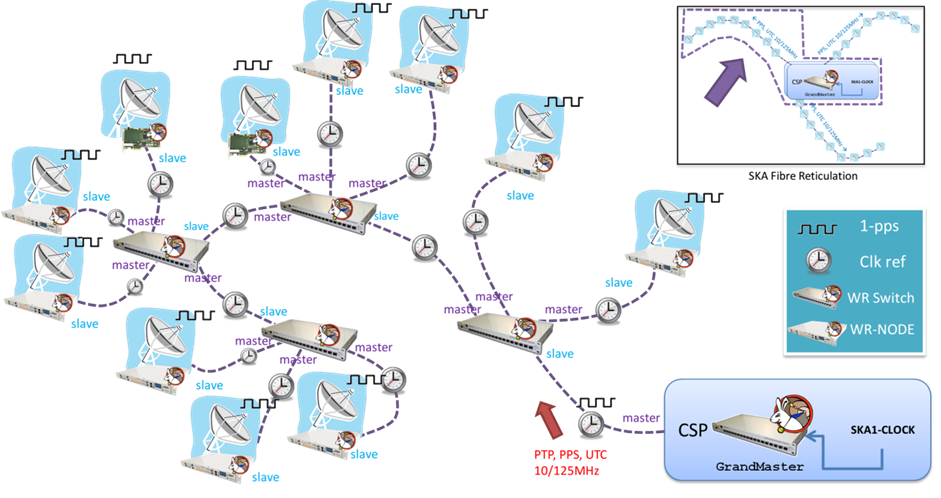
\includegraphics[scale=0.4]{img/ska_pps_network}
\caption{Network topology for PPS signal distribution based on WR switches and
nodes. }
\label{fig:ska_pps_dist_network} \end{figure}

An important feature of the system that must be taken into account is that the PPS pulse at each station is derived from the reference frequency distributed from the SKA clock and not from the WR system. In normal operation, the WR system only monitors the absolute time of each PPS and reports it back activating an alert if the PPS signal is not aligned to the start of the UTC second. This condition indicates a malfunctioning in the timing chain so that the station must discard data to avoid system data corruption. Other functionality associated with the WR part is to temporarily alter the division ratio to bring the PPS edge back in alignment with UTC time. In this case, fringe finding must then be performed to restore the full calibration again.

The centrally located WR switches and the WR end-nodes are connected to a
single strand of single-mode fibre with LC/PC connectors and industry standard
bi-directional SFPs that use two wavelengths (downstream and upstream) to
produce optical signals to be transmitted. Finally the end nodes generate a valid PPS
signal. 

As previously described, this solution requires WR switches and nodes. The
WRS are well-defined equipment with known interfaces and software support. 

For the implementation of the SKA nodes, we have proposed the utilisation of
the WR-ZEN board. Thanks to this new platform, the utilisation of a host
computer/crate to host the FPGA card can be avoided, thus reducing significantly
the equipment price. It is also a remarkable improvement in terms of
dependability which is a key factor taking into account that SKA Telescope
should have an annual availability of about 95\% of the time (although degraded
operation modes can be allowed under some circumstances).  Finally, it is worth to mention that all these features maintain the full flexibility of a complete
CPU+FPGA system on a single board. 

In the following section we describe the proposed node by means of hardware, gateware (FPGA firmware) and firmware that have been developed as a candidate solution for the SKA Telescope PPS distribution system. 

\subsection{A PPS distribution node architecture}
\label{subsec:ska-pps-system-arch}

The PPS distribution system for SKA is based on the WR-ZEN platform that
provides the WR support in order to ensure the synchronisation accuracy in the
system. The first design of the PPS system includes the Fine Delay FMC card
that is used to generate the timing signals through mezzanine channels.
Moreover, it has two Network Interface Cores (NIC) that allows accessing
optical fibre ports as conventional Linux network interfaces. An introduction
to this platform is presented in \cite{migueljl-paper-wr-zen-intro} and a
contribution that improves the NIC bandwidth of the design in
\cite{jorgesg-paper-wr-zen-dma}. In addition, the WR-ZEN is also under study
using other FMC cards such as the FMC ADC card to build a distributed oscilloscope \cite{joselj-paper-wr-zen-adc}.

Nowadays, the utilisation of the Fine Delay FMC card is still under discussion
and there is a possible design which final architecture could be addressed
without this module.

\subsubsection{Hardware} \label{subsec:hardware}

The WR-ZEN board, shown in Figure \ref{fig:wrzen}, is a proprietary design developed in 2015 by Seven Solutions S.L. The major design changes regarding previous WR nodes designs are the inclusion of a Xilinx Zynq FPGA-SoC platform and a flexible and enhanced clocking scheme. The former, enables a more structured design in which software can be organised in abstraction layers. This is achieved by the inclusion of an Linux-like OS, low-level drivers and a
Hardware Abstraction Layer (HAL). These components allow an easy and quick
development of new functionalities on top of all the software that interfaces
with the underlying hardware. Deeper details of the software structure is
presented in section  \ref{subsec:software}. The new clocking circuitry, makes
the new board suitable for many synchronisation applications with diverse
requirements.

\begin{figure}[H] \centering
	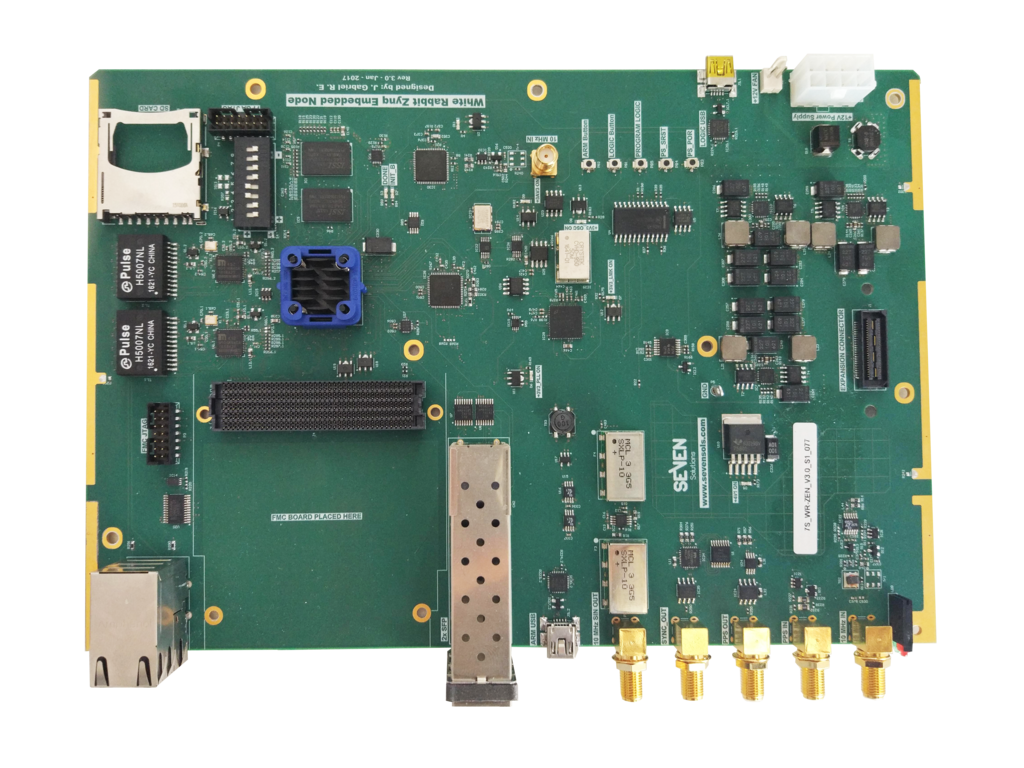
\includegraphics[width=0.7\linewidth]{img/wrzenv3_scaled}
	\caption[WR-ZEN board picture]{WR-ZEN board. Other connectors: Ethernet
	ports, SFP ports and the SMA connectors for the RF input/output
    signals.} \label{fig:wrzen} 
\end{figure}

The FPGA-SoC platform design is composed of two different elements: (i) a
Programmable Logic (PL) including modules described in HDL; and (ii) a
Processing System (PS) formed by all the software executed by an ARM
processor.  The inclusion of the ARM hard-processor in WR node
architectures is a novel approach.  This leads to the utilisation of a powerful
hard-processor unit for software, thereby freeing FPGA resources. In addition
to that, Zynq platforms include the required WR physical components: 
internal programmable PLLs, Gigabit Transceiver Ports (GTPs).
Furthermore, they include not strictly fundamental elements for a WR node design but helpful for future designs such as Ethernet interfaces with hardware timestamp support (allowing PTPv2 support). I/O ports interface with external components used to obtain the time reference from the
main board. The most relevant WR-ZEN I/O interfaces are the FMC HPC
socket (OHWR FMC cards support \cite{ohwr:fmc-fine-delay}), two SFPs sockets, and several external RF connectors for input/output RF and PPS signals.

\begin{figure} \centering
	\includegraphics[width=0.7\linewidth]{img/zenclkschema} \caption[WR-ZEN
	clocking schema]{WR-ZEN new clocking schema. 
	It includes an external PLL to lock to an external
	stable clock reference (GM mode), and a flexible path in the main
	clocks path allowing the final user to choose between a low-noise PLL
	and a full-featured PLL with many options such as programmable output
delays.} \label{fig:zenclkschema} \end{figure}

The extended WR clock schema is depicted in Figure \ref{fig:zenclkschema}.
Besides including new components, the WR-ZEN design, upgrades some of them
in order to provide an increment of the clock stability. All the clock path: Digital to Analogue Converter (DAC), Voltage-controlled crystal oscillator (VCXO), Phase-Locked loop (PLL) have been upgraded. A new DAC \cite{web:ad5541a_datasheet} with a better response time and stability, a low-noise VCXO \cite{web:cvhd950_datasheet} and PLL \cite{web:lmk03806_datasheet}  have been included.
The original PLL \cite{web:ad9516_datasheet} used in previous designs has been maintained because it offers key aspects such as programmable output delays. In order to avoid the development of cascades formed of several PLLs, the signal from the crystal oscillator (XO) is driven to the low-noise PLL first since it allows bypassing its reference to other components without adding noise to the reference. This schema enables using both PLLs at the same time. One of them is used to generate all the WR clocks and the other can be used to generate custom frequencies. The WR general performance is limited by noise when locking to an external reference, in the so called GM mode, described in \cite{Rizzi2016}. It states that, in order to decrease the noise when locking to an external reference, internal PLLs in the FPGA should be avoid. Instead of it, it is recommended to use an analogue external PLL to locks to the external reference generating the necessary clock signals by the internal elements of the WR-logic in the FPGA. Those enhanced features are included in the version 3.0 of the WR-ZEN as shown in Figure \ref{fig:zenclkschema} in order to achieve the expected PPS distribution stability requirements of the SKA project.


\subsubsection{Gateware} \label{subsec:gateware}

The gateware is responsible for configuring the communication between the embedded ARM microprocessor and the FPGA inside the Zynq SoC. 
The main block diagram is shown in Figure \ref{fig:gateware_first_level}. 
It includes the WRPC-2p \cite{torres2016scalability} core that implements the high accuracy timing protocol based on WR and provides basic capabilities, such as Gigabit networking, timestamp mechanisms, debug interfaces, etc. The GTPs include the necessary modules to send/receive packets to/from the network. The NIC are in charge of processing the incoming/outgoing
packets and notify these events to the ARM. The Transmission Time-Stamp Unit
(TxTSU) is an additional module that allows recovering the outgoing packet
timestamps. The Fine Delay core controls the operation of the Fine Delay FMC
card if any is plugged into the FMC socket. The Wishbone (WB) Crossbar
interconnects all the elements of the architecture and eases the configuration
process performed by the ARM. The AXI-WB Bridge is a bus converter between AMBA (Advanced Micro-controller Bus Architecture)
AXI (Advanced eXtensible Interface) and WB. This conversion is necessary because the ARM microprocessor
uses the AMBA specification while others components are based on WB.

\begin{figure}[H] \centering
	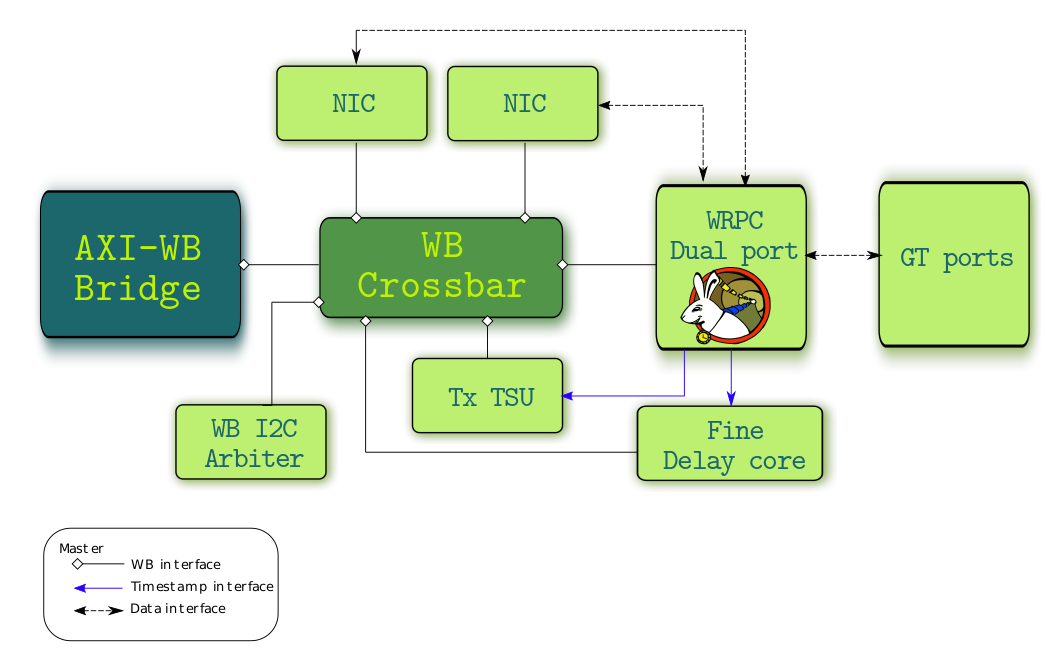
\includegraphics[scale=0.4]{img/gateware_first_level} \caption{Gateware
	project design. WR-ZEN FPGA gateware design. The the WRPC-2p core that is responsible for implementing the WR protocol. The GT ports allows to transmit/receive packets to/from the network through the optical SFP modules. The NIC cores manage Ethernet packets and behave as standard network interface cards for the ARM microprocessor. The AXI-WB Bridge translates AXI transactions into WB ones. It is important because the ARM is connected using AMBA specification meanwhile the WR FPGA cores use Wishbone bus standard. Finally, the Fine Delay core contains the necessary resources to control the Fine Delay FMC card.} \label{fig:gateware_first_level} 
\end{figure}

\subsubsection{Firmware} \label{subsec:firmware}

The firmware code performs all the WR functionalities. 
In the node architecture, the embedded software part of the WR protocol together with some device drivers runs in the soft-microprocessor described in the previous section. The main tasks of the WR routines are the servo loop algorithm, which maintains the local oscillator locked to the recovered master's frequency, and the implementation of the WR-PTP stack. In addition, a simple Command Language Interface (CLI) has been integrated in the platform to allow user interaction in standalone configurations.

\subsubsection{Software} \label{subsec:software}

The WR-ZEN is the first WR node taking advantage of a Linux based OS in a standalone configuration.  
Due to the inclusion of a dual-core ARM microprocessor, the system design is not longer tied to low-level software implementations. New functionalities, such as communication protocols, management tools, etc., are quickly added thanks to the support provided by the OS. The hardware abstraction layer and drivers help to abstract the management of the associated logic. This middleware adds also more security access to the hardware.

The software components are presented in Figure
\ref{fig:software_architecture}. Software is divided into the userspace utilities and the kernel support. The userspace utilities includes the \textit{Zen library} that implements the basic functionalities for the \textit{Zen tools} through the C standard library. The \textit{Zen tools} provide some mechanisms to program the FPGA design and connect to the internal UART for debugging/configuration tasks among others.  Moreover, other utilities are included to control the Fine Delay FMC card if plugged.

In the kernel side, some drivers have been implemented. The main one is the
\textit{zen} driver that is responsible for setting up all the IP cores in the
FPGA and creates the standard Linux network interfaces. The \textit{fmc} and
\textit{zio} drivers are retrieved from the OHWR repository and implements a
generic support for FMC and ZIO buses respectively.  The \textit{zio} driver
has been modified in order to work properly in the WR-ZEN platform.  The
\textit{zen-nic} kernel module is in charge of enabling/disabling network
capabilities of the \textit{zen} driver. The \textit{fmc-fine-del} driver
provides basic functionalities for the Fine Delay FMC card.

As previously mentioned, there are dependencies between the different kernel
drivers. The \textit{zen} driver depends
on \textit{fmc}. The \textit{fmc-fine-del} needs \textit{zen}, \textit{zio} and
\textit{fmc}. The \textit{zen-nic} only uses the \textit{zen}.

\begin{figure}[H] \centering
	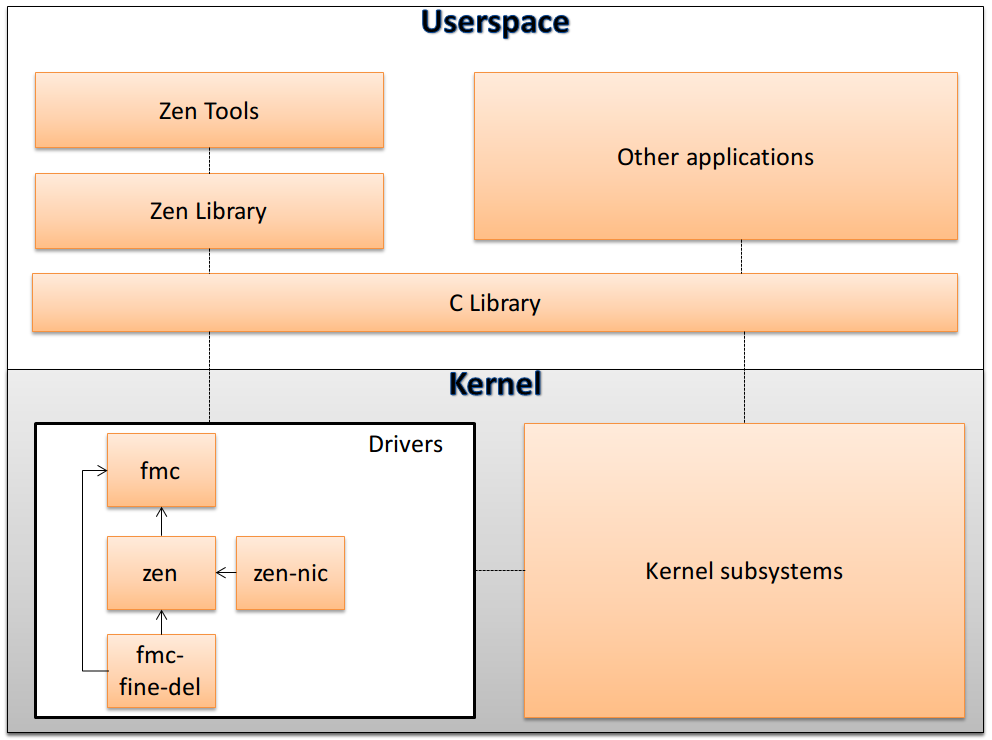
\includegraphics[scale=0.4]{img/software_architecture}
	\caption{WR-ZEN software
	architecture. It is based on Linux kernel, in which
	several tools and drivers have been developed to manage the WR functionality. The
	tools can be used to program the FPGA, update the soft-microprocessor
	code or connect to the virtual UART interface of the WRPC-2p. They call
	the Zen Library procedures that use C Library functions and
	switch to kernel mode through system calls. In the kernel space, the
	drivers are responsible for implementing all the requested functionalities. }
	\label{fig:software_architecture} 
\end{figure}

The next section describes the main performed experiments and the obtained
results using the WR-ZEN.

